\section{Agent-Coordinated Task-Level Operation}
\label{sec:closed-loop-operation}

\begin{figure*}[!t]
\centering
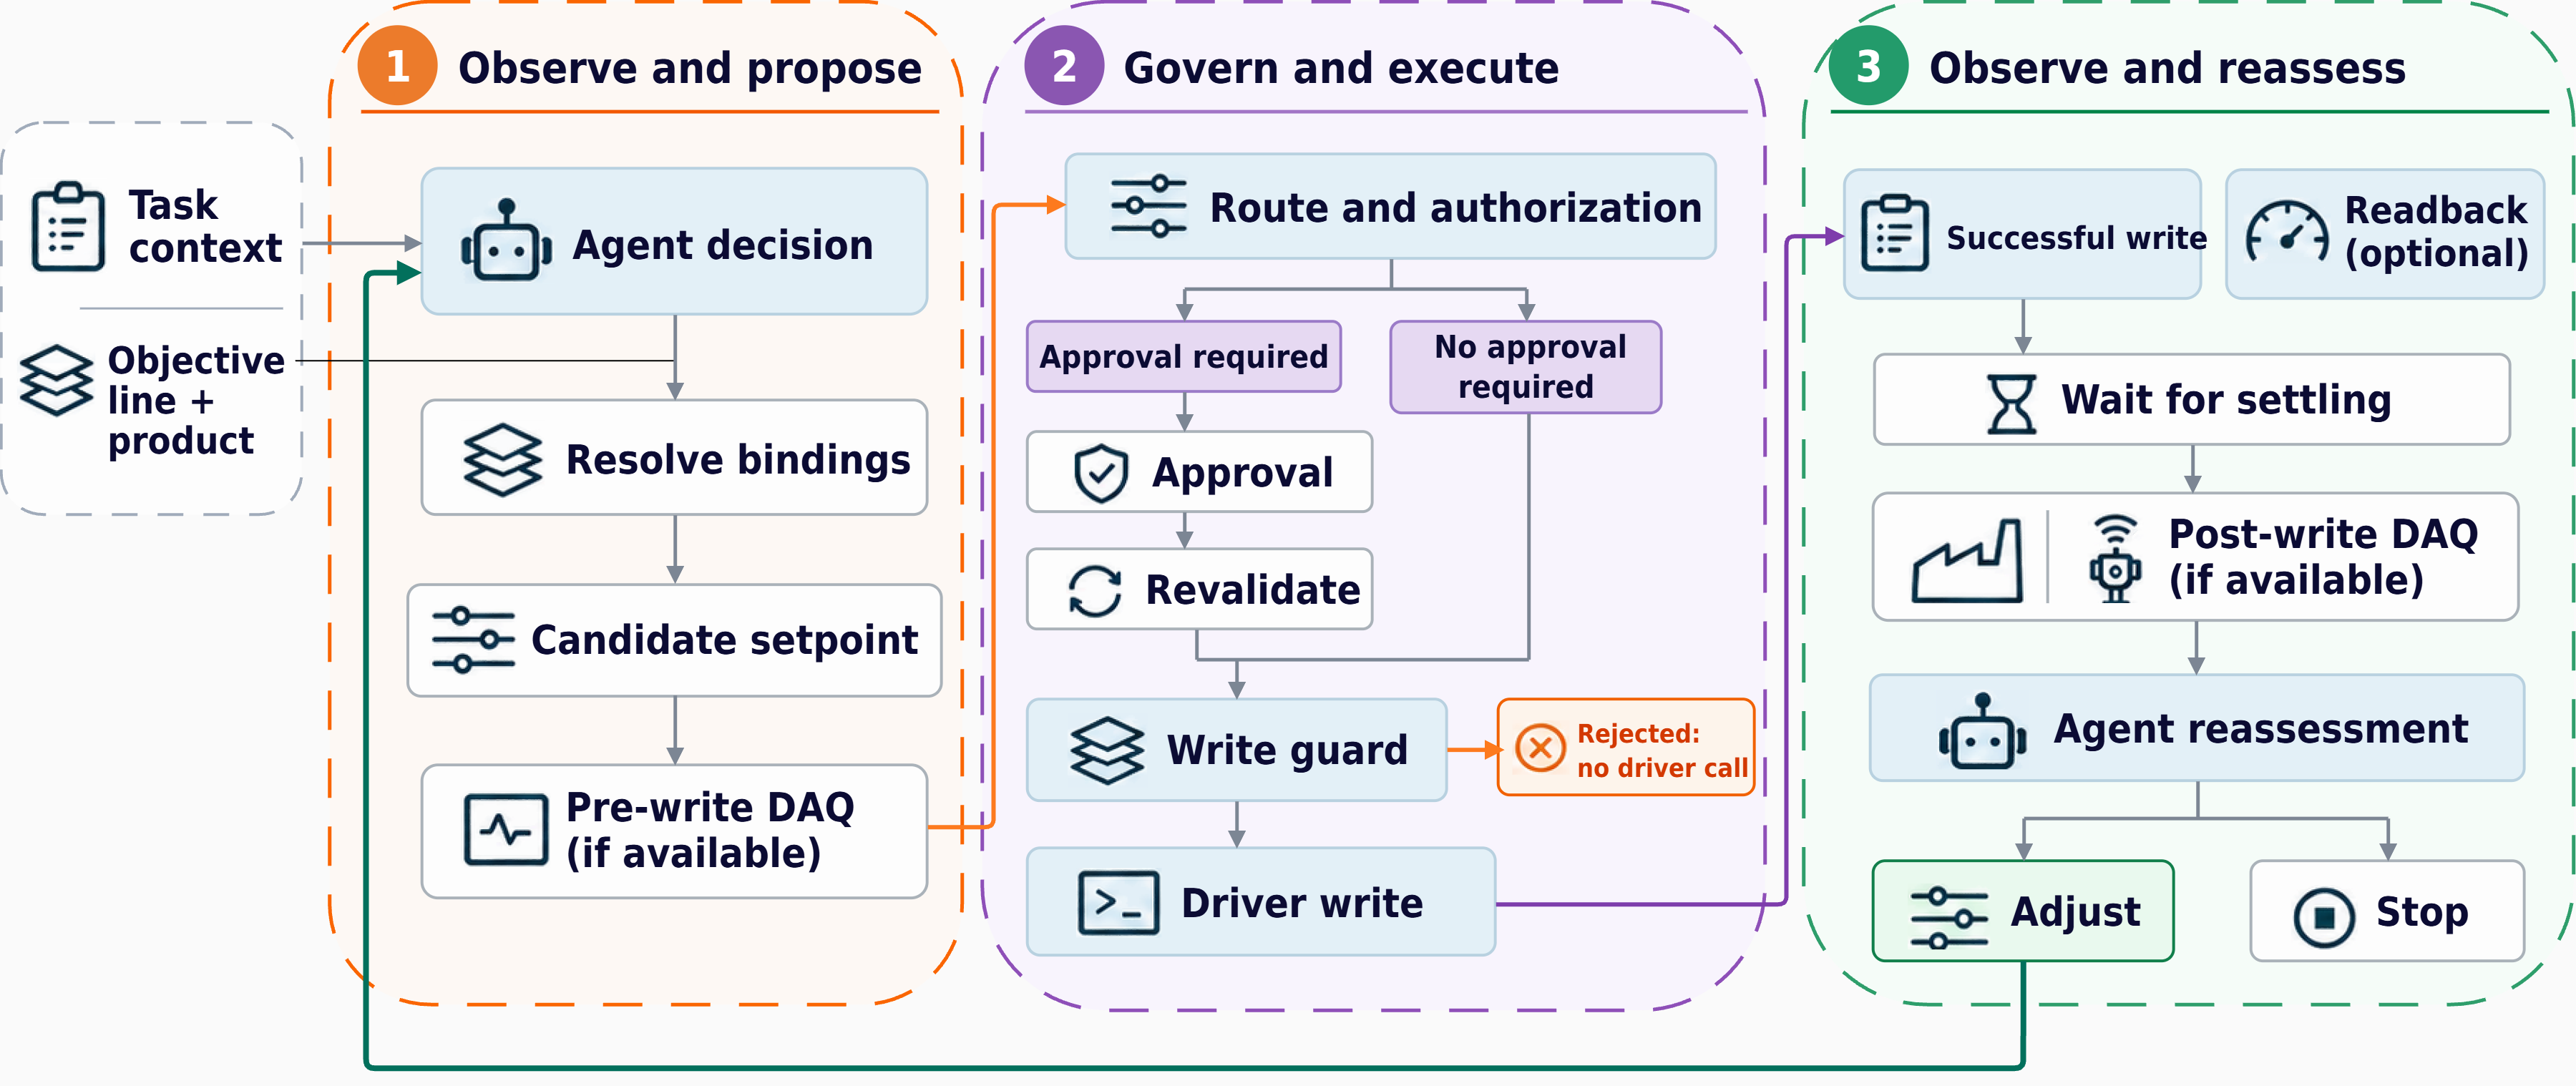
\includegraphics[width=\textwidth]{resources/fig3.png}
\caption{Conceptual task-mediated setpoint exploration. Observations used in the initial agent decision are not shown; the optional pre-write DAQ read follows candidate formation. If approval is required, the route revalidates the request after approval. Both routes remain subject to authorization and write guards. Pre-dispatch rejection does not reach the driver. The right panel shows the success path: any readback is distinct from the later DAQ read, and waiting does not establish that the process has settled. Adjusting or stopping requires a subsequent agent decision. Approval denial and driver errors are not shown.}
\label{fig:agent-loop}
\end{figure*}

Section~\ref{sec:design} defined the entry paths and the shared dispatch checks. Fig.~\ref{fig:agent-loop} follows the intended task-mediated turn: propose an adjustment, check and execute the request, then reassess the result. It illustrates the \texttt{optimization\_explore} workflow, not an end-to-end trial reported in Section~\ref{sec:eval}. A task supplies an objective and production context. The agent can use configured DAQ or other read-only observations to form a typed adjustment; neither the data nor the context grants write authority. The control node comes from \texttt{control\_node\_id} or a configured binding; the DAQ target comes from an explicit ID or agent DAQ binding.

In goal mode, a lead agent may decompose the objective and dispatch worker subtasks. For an exploration step, the responsible agent may invoke \texttt{optimization\_explore}, which resolves the DAQ target, checks bindings, and submits a candidate before device I/O.

The operation resolves the applicable limit profile and control binding, then reads the stored value as $u_0$; this is not necessarily a fresh readback. The agent combines this state with its objective and direction. If direction is omitted, the operation defaults to an upward adjustment; otherwise $s\in\{-1,+1\}$. For a step $\Delta u$, it forms
\begin{equation}
 u^{*}=\operatorname{clip}\!\left(u_0+s\Delta u,\,u_{\min},\,u_{\max}\right).
 \label{eq:optimization-candidate}
\end{equation}
In Eq.~(\ref{eq:optimization-candidate}), configured tuning bounds take precedence; node bounds are used otherwise. The effective step is selected in this order: an explicit argument, the binding's tuning step, the scene's maximum step, or one twentieth of the node range.

Before entering the governed write path, the operation resolves the DAQ target and checks visibility. The current implementation also includes identifiability and model--ontology checks added after the reported experiments. If the applicable pre-write checks pass, the operation attempts a pre-write DAQ read; its mean may be unavailable.

A valid candidate enters the governed single-node write path in Algorithm~1: a pre-dispatch denial stops the request before any driver call, whereas a driver-stage error may occur after dispatch has begun, so status alone cannot establish whether the device changed and state must be reconciled before retrying.

After a successful write, the operation waits 10--300~s (45~s default) and attempts a post-write DAQ read before returning the exploration result. The observation windows are $[t_0-\tau,t_0]$ and $[t_0,t_1]$, where $t_0$ is an operation timestamp taken before the pre-write read and any approval wait, $\tau$ the pre-write window length, and $t_1$ the post-write read time. Because dispatch can occur after $t_0$, the second window may include pre-dispatch samples, so the resulting mean is not causal. The earlier implementation used trailing 45-s windows.

The exploration record stores the target, step, available DAQ means, and write status; the shared path separately records the command outcome and any available readback. The operation then returns an exploration summary. On a later turn, the agent can inspect the returned evidence, choose another step, or stop; iteration always requires a subsequent agent decision.


